\documentclass[tikz, margin=0.1pt]{standalone}
\usepackage{tikz} 

\begin{document}

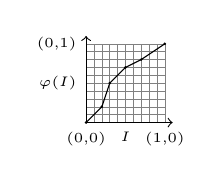
\begin{tikzpicture}[scale=1, dot/.style = {circle, fill, minimum size=#1, inner sep=0pt, outer sep=0pt}, dot/.default = 1pt] 

% Grid
\draw[step=0.1,gray,very thin] (0,0) grid (1,1);  % Adjust step for more/less gridlines

% Axes
\draw[thin,->] (0,0) -- (1.1,0);
\draw[thin,->] (0,0) -- (0,1.1);

% Points
\node[anchor=north] at (0.5, 0) {\tiny $I$};
\node[anchor=east] at (0,0.5) {\tiny $\varphi(I)$};
\node[anchor=north] at (0,0) {\tiny (0,0)};
\node[anchor=east] at (0,1) {\tiny (0,1)};
\node[anchor=north] at (1,0) {\tiny (1,0)};

% Dots and lines
\node[dot] at (0,0) {};
\node[dot] at (.2,.2) {};
\node[dot] at (.3,.5) {};
\node[dot] at (.5,.7) {};
\node[dot] at (.7,.8) {};
\node[dot] at (1,1) {};
\draw[thin] (0,0) -- (.2,.2) -- (.3,.5) -- (.5,.7) -- (.7,.8) -- (1,1);

\end{tikzpicture}

\end{document}
